\chapter{Background}
In this chapter, a more thorough introduction to the research topic of this project is presented while also discussing related work in the area and introducing the Machine Learning concepts and techniques used.
\section{Hit Song Science}
Perhaps unsurprisingly, this research topic is quite a popular subject that has also gained some attention from the media. This is probably because a few companies have released products that they claimed were able to predict hit songs with high accuracy. This, as you can imagine, would be an invaluable tool for music producers and artists alike since they would be able to use it to their advantage and ultimately make a profit. However, it is unclear if those hit prediction tools actually worked and the implementation details were mostly kept secret.

This field of investigation has been referred to as Hit Song Science, a term coined by Mike McCready, founder of a music analysis company, and it aims to predict the success of songs before they are released on the market. However, as it turns out, there might be more to predicting the popularity of songs than just the features of the audio itself. Psychological aspects also come into play and a wide range of factors such as exposure, music marketing, media broadcasts, social influence play a role in whether we like a song or not. That is because what we listen to might be influenced by what our friends listen to, by what is played on radio/television or by what is being more heavily marketed. It is also usually the case that songs of popular artists will also be popular since they already have the exposure, while a new, unknown artist might struggle to get their songs on the radio since the popular songs get all the airtime (the rich get richer and poor get poorer). 

This makes the whole prediction problem even more complex than it was already. However, in Hit Song Science and, consequently, in this project, the goal is to look at the relation between features of the audio and the popularity of that song while disregarding these aforementioned complex and confusing psychological aspects. This problem then becomes similar to the prediction of stocks or the weather. Another way to look at this, as Pachet, puts it is "...as an idealistic attempt to determine the 'objective causes' of individual music preference, independently of the effects of social influence"  \cite{li_music_2011}.

\section{Related work}
\label{sec:relatedwork}
Research in this area has gone back and forth over time with some studies claiming that this kind of prediction might be possible and others saying that it is not. One of the earliest attempts is the work of Dhanaraj and Logan \cite{dhanaraj2005automatic}. They used general acoustic features (based on Mel-frequency cepstral coefficients) and features extracted from lyrics. To classify hits they used Support Vector Machines (SVMs) and boosting classifiers and for the data they used a database of 1700 songs. After the study, they concluded that there might indeed be something that distinguishes hits from non-hits and that audio based features and lyrically based features perform well on their own, but result in poorer performance when combined. 

Later, a larger scale and more complete study by Pachet and Roy \cite{pachet2008hit} contradicted their results. They used a database of 32000 songs with features from the MPEG-7 audio standard, a specific acoustic set generated with proprietary algorithms and a set of high-level metadata manually produced by humans. The classifier used was also SVM with an RBF kernel so the main differences were the features used and the size of the dataset. This study concluded that the popularity of songs cannot be learned from features of music titles, in this way contradicting the claims of Hit Song Science. This experiment could have put end to the debate on the topic due to its scale and level of completeness but as it turns out it might have had the opposite effect, fuelling even more experiments since it did not disprove the hypothesis completely \cite{li_music_2011}.

\begin{figure}[h]
\centering
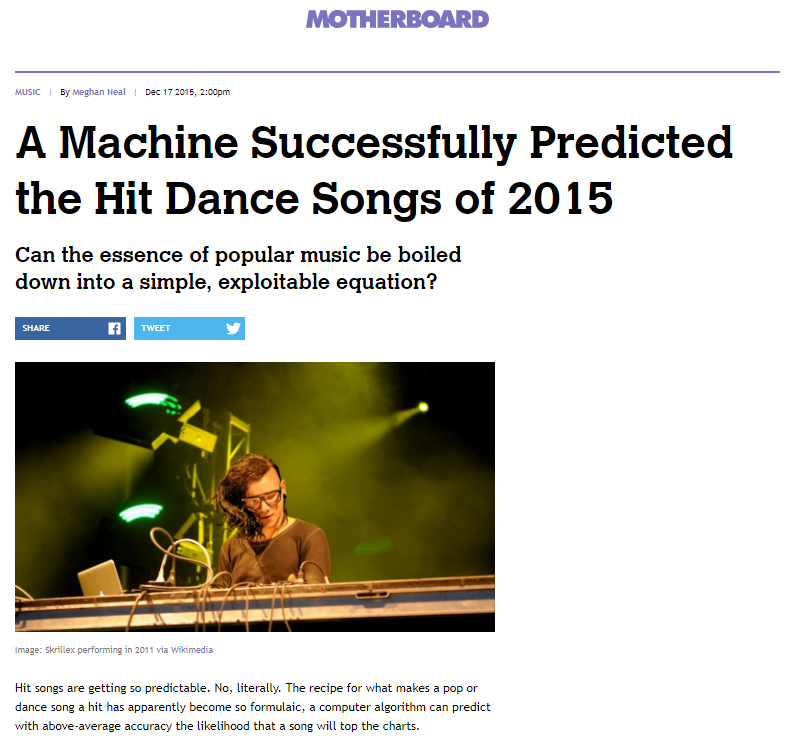
\includegraphics[width=0.50\linewidth]{background/fig/art2.PNG}
\caption{Online artice about the study of Herremans et al. \cite{herremans2014dance} \cite{MachineArticle:online}}
\label{fig:hitarticle}
\end{figure}

Trying to distinguish the top 5 from top 30-40 hits, Ni et al. \cite{ni2011hit} showed an experiment with more optimistic results due to the slightly different approach, the more novel audio features used (extracted from the EchoNest API, a music intelligence platform) and the classifier (a time-shifting perceptron). They claimed that hit song science might be a science once again. The research, however, does not include a lot of the perhaps important details of the implementation. Another study was conducted by Herremans et al. \cite{herremans2014dance} that looked at a similar approach, trying to predict if a song is a top 10 dance hit. Therefore, it only focused on a particular genre. The features were also obtained from The Echo Nest. They used models such as C4.5 trees, RIPPER rule set, logistic regression and SVMs, the best performing being the logistic regression model. This experiment again showed promising results concluding that predicting the popularity of dance songs is possible and is due to only using recent songs (so there is no need to account for the change in music taste over time), focusing on one genre and the features used.

More recently, Pham et al. \cite{pham2016predicting} used a subset of 2700 tracks from The Million Song Dataset \cite{bertin2011million} with features from this data set plus some from The Echo Nest. They compared different classifiers concluding that the SVM with an RBF kernel was the best performing one. Their aim was to also find the features that were more prominent in the prediction. Again, their study showed good results and the features that were more powerful predictors seem to have been the metadata ones rather than the acoustic ones since they seemed to reflect the trait of a song more accurately. An even more recent research by Reiman and Ornell \cite{reiman2018predicting} took an approach similar to the one in this project. They looked at predicting hit songs using four different classifiers with a data set of 600 tracks from the Billboard Hot 100 charts and features from the Spotify API. Their results were not as good as some of the previously presented experiments but were still slightly better than a random predictor.

\begin{figure}[h]
\centering
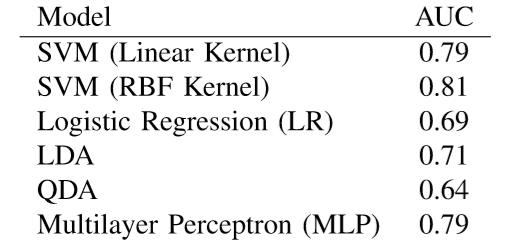
\includegraphics[width=0.7\linewidth]{background/fig/pic1.PNG}
\caption{Classifier AUC score results from the study of Pham et al. \cite{pham2016predicting}}
\label{fig:pham1}
\end{figure}

The results of these experiments seem promising overall making pursuing a different approach at this task worthwhile. While each research seems to have taken a slightly distinct path there were still certain common points. A few papers looked at models such as SVMs, logistic regression, naive bayes, multilayer perceptron, k-nearest neighbors and used features from The Echo Nest. This was a good starting point for my own study.

\section{Classification algorithms}
It seems clear now that some sort of prediction needs to be performed. To do that, this project uses machine learning which is used for the finding of patterns in data in an automated manner \cite{shalev2014understanding}. Nowadays,  we probably encounter machine learning every day when we search the internet, when shop online, even our phones might use it for unlocking using face recognition. It is truly all around us. 

But how do machines learn? Well, in a way similar to how animals or humans do, by using past experience to determine what to do in a new situation. In a very simple example of machine learning, that of filtering spam emails, the machine learning algorithm will be provided with a lot of examples of spam and non-spam messages. It will find patterns in these messages, such as the frequent occurrence of bad words in spam perhaps and when a new email arrives it will be able to tell if it is spam or not by using its 'past experience'. There are two main types of ways in which a machine can learn: supervised and unsupervised. 

Supervised learning applies in situations like the ones described above with the spam filter. Given a sample of messages that are labelled as spam and some labelled as not spam, when a new message arrives it can be labelled according to its similarity to a spam/non-spam message. In Figure \ref{fig:supunsup} a line (usually called a decision boundary) is drawn to separate the two classes. When a new point is plotted, it will be labelled according to which side of the decision boundary it is on.

On the other hand, in an unsupervised task the messages used for training are not labelled and so the algorithm needs to find patterns that separate the messages in a way, by clustering the data set into smaller subsets of similar messages, for example, like in Figure \ref{fig:supunsup} \cite{shalev2014understanding}. 

\begin{figure}[h]
\centering
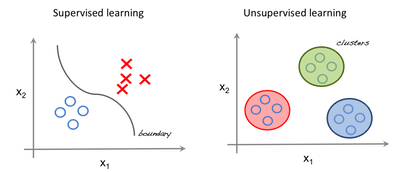
\includegraphics[width=0.9\linewidth]{background/fig/graph.png}
\caption{Supervised and unsupervised learning visualised \cite{SupervisedUnsupervised:online}}
\label{fig:supunsup}
\end{figure}

For the task in this project supervised learning will be used since we will provide the machine learning models with examples of songs that are labelled as popular or not popular. The model should then learn a certain pattern that differentiates popular songs from the less popular ones that it will then be able to apply to a previously unseen song and label it accordingly. 

As a starting point for choosing which classification algorithms to use, the related literature was reviewed. A few research papers used Support Vector Machines, Logistic Regression, Gaussian Naive Bayes, Multi-layer Perceptron and even K-Nearest Neighbours. Those were implemented to be able to compare results with previous work but other models were also tested such as Random Forests and AdaBoost. Below a succinct description of these models is provided.

Logistic regression is a machine learning technique that came from the field of statistics. It is at its core a mathematical modelling approach used to describe the relationship between a set of independent variables and a dependent variable. It is a very popular model because its output is a value between 0 and 1, value which describes a probability since it uses a sigmoid function (Equation \ref{eq:logreg}) to map predicted values to probabilities. The output represents the likelihood of the example belonging to class 1. For example, if predicting whether an individual has a disease or not, the probability will indicate how likely it is that the individual has that disease \cite{kleinbaum2002logistic}.

\begin{equation}
f(z)=\frac{1}{1+e^{-z}}
\label{eq:logreg}
\end{equation}

\addvbuffer[12pt 8pt]{
\begin{tabular}{lll}
	where & $e$ & is Euler's number,\\
	& $z$ & is the input to the function(the algorithm's prediction).\\

\end{tabular}
}


K-Nearest Neighbours is one of the simplest algorithms in machine learning, yet it is quite effective. To predict the class of a new given point, it looks at its k nearest neighbours (where k can range from 1 to the total number of points minus one and is usually chosen depending on the data). It then uses a majority vote to decide on the class of the new point \cite{16Neares99:online}.

Support Vector Machines are a "machine learning tool used for learning linear predictors in high dimensional feature spaces" \cite{shalev2014understanding}. It tries to find an optimal hyperplane to separate the given classes. The hyperplane is optimal when the distance between the hyperplane and the training examples is maximum. For example, in two dimensions the hyperplane would be a line that separates the points as seen in \autoref{fig:svm} and in three dimensions it would be a plane \cite{Introduc22:online}.

\begin{figure}[h]
\centering
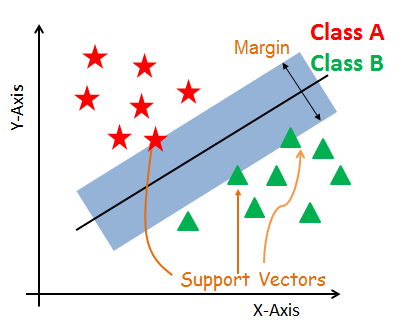
\includegraphics[width=0.6\linewidth]{background/fig/svm.PNG}
\caption{SVM application on 2D data \cite{SVMGraph:online}}
\label{fig:svm}
\end{figure}

The multi-layer perceptron (MLP) is a type of artificial neural network. As the name suggests, it is built upon the simpler perceptron which is a linear classifier that models a biological neuron. A multi-layer perceptron is composed of more than one perceptron which makes it able to solve more than just linear prediction tasks. An input layer receives the signal (the input data) and an output layer makes a decision based on the input. Between those two layers there can be any number of hidden layers that handle the bulk of the computation \cite{ABeginne87:online}.

The Naive Bayes classifiers are a family of simple probabilistic classifiers. Despite their simplicity they are very popular and have proven very effective. They use Bayes' theorem but with the added naive assumption that all the features are independent of each other, in other words, they assume conditional independence. This is considered a "naive" approach because it very rarely applies to the real world \cite{zhang2004optimality}. Gaussian Naive Bayes comes as an extension of the naive Bayes that adds the capability of handling continuous variables by making the assumption that the features are generated using a single Gaussian distribution \cite{john1995estimating} \cite{reiman2018predicting}.

The Random Forest or Random Decision Forest is an ensemble learning method, which means it uses multiple classifiers, in this case decision trees, to classify the data and then takes a majority vote of all those classifiers to decide on the class of an example. In this way, it mitigates the tendency of decision trees to overfit the data, improving the generalisation accuracy \cite{ho1995random}.

The AdaBoost classifer \cite{freund1997decision}, short for Adaptive Boosting, is a machine learning ensemble meta-algorithm that essentially tries to obtain a strong classifier from a set of weak ones. It trains a classifier on the data set and then creates new instances of that classifier that are trained on the same data set but the weights of incorrectly classified instances are adjusted (hence the adaptive title) \cite{sklearnadaboost:online}.

These algorithms were then implemented using the \textit{sci-kit learn} library \cite{pedregosa2011scikit} in Python. It is a module for machine learning that features various classification, regression and clustering algorithms including the ones mentioned above but also many more. Furthermore, it is designed to work with other numerical libraries in Python such as NumPy and SciPy. The code is run using Jupyter Notebooks \cite{kluyver2016jupyter}, a document format in which code from different languages can be executed. It is based around the IPython kernel which can run the Python code in Jupyter. It works in a browser and it provides a way of integrating code, explanations (in the form of text) and results (in the form of plots or graphics) in a single document which makes for easy reading, executing and understanding.

\section{Feature selection}

Feature selection is the process of removing the features that are not helpful to the predictor from the data. Often times this can improve the performance of the model since features that are not relevant can have a negative impact on the predictions. We are interested in only keeping the features that have the highest contribution to the desired output \cite{FeatureSel:online} \cite{guyon2003introduction}. There are three main types of methods used for feature selection: wrapper methods (use the model to score different feature subsets), filter methods (select feature subsets in the preprocessing phase, without using the model) and embedded methods (specific models can perform feature selection as part of training). 

Since the data only has 13 features the best feature subset can be found searching exhaustively by calculating a score for every possible feature combination and picking the best one. This is a wrapper method. There are therefore \(2^{13} - 1\) possible feature subsets and for each of them an AUC score is calculated using cross validation. Then the process is repeated for every model since the features chosen depend on the model used. The algorithm then looks like Algorithm \ref{alg3}.

\begin{figure}[h]
\centering
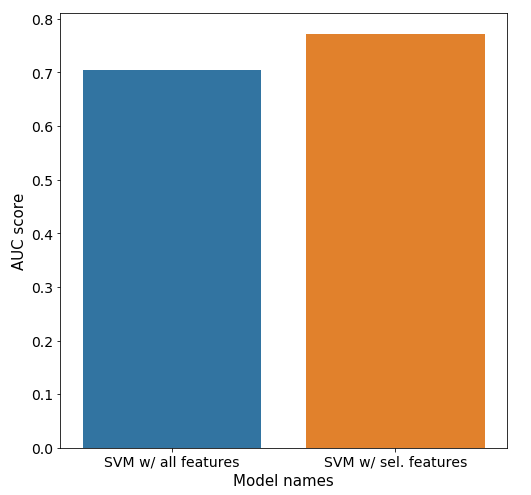
\includegraphics[width=0.8\linewidth]{background/fig/fs1.PNG}
\caption{AUC score for SVM before and after feature selection}
\label{fig:fs1}
\end{figure}

As an example, the performance increase for SVM can be seen in Figure \ref{fig:fs1} with the score plotted for the classification being performed on data with all the 13 features and on data with 7 selected features (energy, tempo, speechiness, instrumentalness, time signature, duration, loudness). It is about a 7\% increase which may not be much but the reduction of features leads to a much simpler model, the number of features being almost halved.

\begin{algorithm}[caption={"Feature selection algorithm"}, label={alg3}]
begin
    foreach model in the model list
      foreach possible feature subset
        do cross validation
          calculate AUC score for each iteration
        end
        calculate average AUC score for all iterations
        store feature set and score in a list
      end
      pick subset with best score for model
    end
end
    
\end{algorithm}

\section{Imbalanced classes}
\label{sec:imbalance}
Early on when trying to evaluate the models the results seemed unusually high. That was because I was only looking at the prediction accuracy of the models which is the percentage of correct predictions. That was a problem since almost 90\% of the data set is of class 0 and only 10\% of class 1 so it is highly imbalanced (this can be observed in Figure \ref{fig:imbalance}). This meant that if the model predicted everything as class 0 it would have a 90\% accuracy even though it failed to identify any of the hits which is what we are actually interested in. To mitigate this problem a few different approaches were tried: using over-sampling, adjusting class weights in models and looking at different scoring metrics (discussed in Section \ref{sec:evalation}).

\begin{figure}[h]
\centering
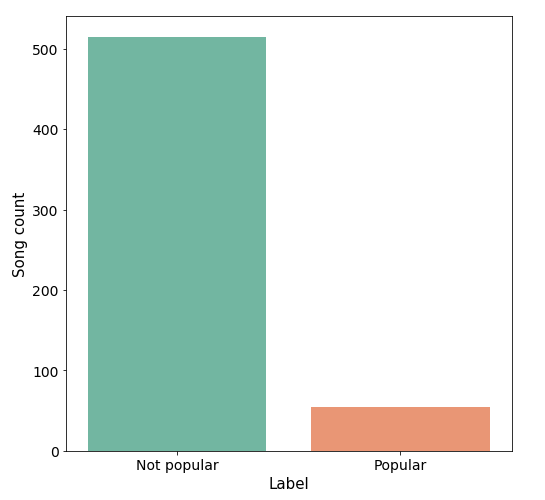
\includegraphics[width=0.7\linewidth]{background/fig/imbalance.PNG}
\caption{Plot of number of examples for each class in the data set}
\label{fig:imbalance}
\end{figure}

Over-sampling is a technique used to create more examples of the minority class to make the data set balanced. A common way to do so was to just duplicate the examples of the minority class, but this can easily lead to overfitting. A better approach is SMOTE (Synthetic Minority Over-sampling Technique) \cite{chawla2002smote}, a technique used to create new "synthetic" samples by using an algorithm similar to k-nearest neighbours that creates a new example and randomly sets its feature values based on those of the neighbours. 

Another technique that can be used to mitigate this problem involves adjusting the model to penalise a misclassification of a sample of class 1 more than one for class 0. This can be done by adjusting the weights of the classes and some models in sci-kit learn support a parameter that sets the weights automatically according to the balance of samples in the data set.

Both of these options were used and compared to ensure the best solution was chosen. The scores were similar with slightly higher results when adjusting the weights but since that was not available for every model, over-sampling also had to be used. 

